\documentclass[12pt]{article}
\usepackage{latexblog}

% ============================================================
% Blog Metadata
% ============================================================
\blogtitle{SQLite3 文件格式分析}
\blogdate{2020-09-25}
\blogtags{Sqlite3, 闲话编程, 存储}
\bloglang{zh}
\blogsummary{}

\begin{document}
\makeblogtitle

最近一直在思考如何使用btree文件结构做一个单文件的加密存储格式，因此研究了一下sqlite3的文件格式以为参考。

\section{文件布局}\label{ux6587ux4ef6ux5e03ux5c40}

每一个sqlite的数据库文件由1个或者多个大小相同的页（page）构成，其文件布局如下：

\begin{figure}
\centering
\pandocbounded{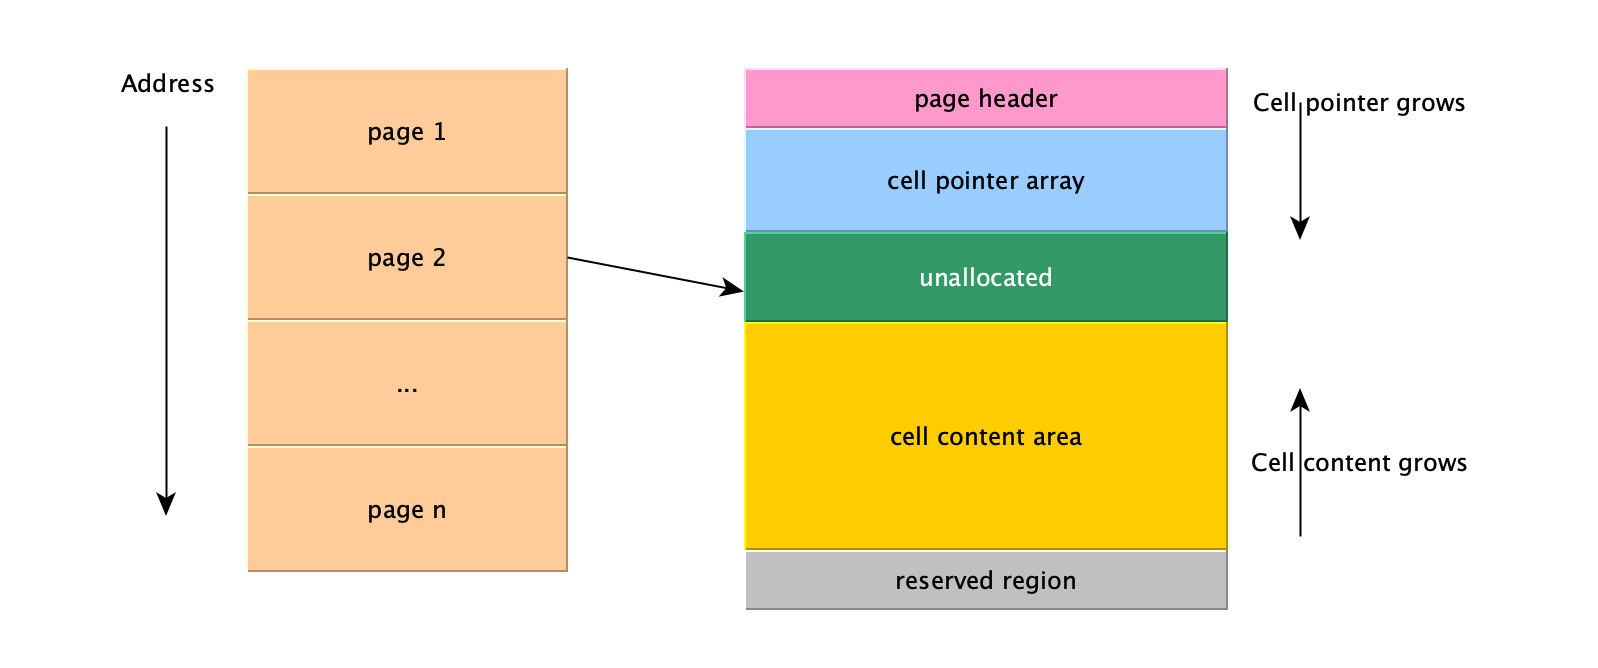
\includegraphics[keepaspectratio,alt={Sqlite3 file layout}]{images/Sqlite3-file-layout.png}}
\caption{Sqlite3 file layout}
\end{figure}

其中，第一个page记为page 1（而不是从0开始算）。任一个page都属于以下的某一种：

\begin{itemize}
\tightlist
\item
  lock-byte page，设计给VFS使用，本身sqlite并不需要，任何大小在1073741824(1024m=1G)以内的数据库文件都不包含lock-byte page。
\item
  freelist page，数据库的空闲page（譬如删除一些数据之后，页仍然保留）

  \begin{itemize}
  \tightlist
  \item
    freelist trunk page，存储一个4位的leaf page数组，因最小的page可用空间为480所以至少可以存储120个entry。其中第一个id为下一个freelist trunk page的id，如果没有则为空
  \item
    freelist leaf page，不包含任何信息
  \end{itemize}
\item
  b-tree page

  \begin{itemize}
  \tightlist
  \item
    table b-tree interior page
  \item
    table b-tree leaf page
  \item
    index b-tree interior page
  \item
    index b-tree leaf page
  \end{itemize}
\item
  payload overflow page
\item
  pointer map page
\end{itemize}

\section{页（page）}\label{ux9875page}

\subsection{页大小（page\_size）}\label{ux9875ux5927ux5c0fpage_size}

页的大小必须为512\textasciitilde65536间的2的整数幂。从\href{https://www.sqlite.org/releaselog/3_12_0.html}{3.12.0}开始，默认的page大小从1024调整到了4096。可以通过如下的命令来查看当前数据库的页大小：

\begin{Shaded}
\begin{Highlighting}[]
\ExtensionTok{sqlite}\OperatorTok{\textgreater{}}\NormalTok{ pragma page\_size}\KeywordTok{;}
\ExtensionTok{4096}
\ExtensionTok{sqlite}\OperatorTok{\textgreater{}}\NormalTok{ pragma page\_count}\KeywordTok{;}
\ExtensionTok{3}
\end{Highlighting}
\end{Shaded}

可以通过命令来设置page\_size，不过必须在创建库之前操作，否则不能生效。

\begin{Shaded}
\begin{Highlighting}[]
\ExtensionTok{hfli@192:btree/sqlite}\NormalTok{ $ sqlite3 p512.db}
\ExtensionTok{SQLite}\NormalTok{ version 3.28.0 2019{-}04{-}16 19:49:53}
\ExtensionTok{Enter} \StringTok{".help"}\NormalTok{ for usage hints.}
\ExtensionTok{sqlite}\OperatorTok{\textgreater{}}\NormalTok{ pragma page\_size}\KeywordTok{;}
\ExtensionTok{4096}
\ExtensionTok{sqlite}\OperatorTok{\textgreater{}}\NormalTok{ pragma main.page\_size=512}\KeywordTok{;}
\ExtensionTok{sqlite}\OperatorTok{\textgreater{}}\NormalTok{ pragma page\_size}\KeywordTok{;}
\ExtensionTok{512}
\end{Highlighting}
\end{Shaded}

然后我们创建一个简单的表，来一探数据库文件的究竟：

\begin{Shaded}
\begin{Highlighting}[]
\KeywordTok{create} \KeywordTok{table}\NormalTok{ person(}
    \KeywordTok{id} \DataTypeTok{integer} \KeywordTok{not} \KeywordTok{null} \KeywordTok{primary} \KeywordTok{key}\NormalTok{,}
\NormalTok{    name text,}
\NormalTok{    age }\DataTypeTok{number}\NormalTok{,}
\NormalTok{    remark text}
\NormalTok{);}
\end{Highlighting}
\end{Shaded}

创建完成后，不插入数据，则文件中共有三页，

\begin{Shaded}
\begin{Highlighting}[]
\DecValTok{53514}\ErrorTok{C69746520666F726D617420330002000101004020200000000100000003}
\OperatorTok{...}
\DecValTok{0100000000000000000000000000000000000000000000000000000000000000} 
\OperatorTok{...}
\DecValTok{0}\ErrorTok{D00000000020000000000000000000000000000000000000000000000000000}
\OperatorTok{...}
\end{Highlighting}
\end{Shaded}

\subsection{文件头}\label{ux6587ux4ef6ux5934}

数据库文件的第一个页为一个特殊的页，其中包含的是数据库的文件头。上述的数据库文件头为：

\begin{Shaded}
\begin{Highlighting}[]
\DecValTok{53514}\ErrorTok{C69} \DecValTok{74652066} \DecValTok{6}\ErrorTok{F726D61} \DecValTok{74203300} \DecValTok{02000101} \DecValTok{00402020} \DecValTok{00000001} \DecValTok{00000003}
\DecValTok{00000000} \DecValTok{00000000} \DecValTok{00000001} \DecValTok{00000004} \DecValTok{00000000} \DecValTok{00000003} \DecValTok{00000001} \DecValTok{00000000}
\DecValTok{00000000} \DecValTok{00000000} \DecValTok{00000000} \DecValTok{00000000} \DecValTok{00000000} \DecValTok{00000000} \DecValTok{00000000} \DecValTok{00000001}
\DecValTok{002E3420} \DecValTok{0}\ErrorTok{D000000} \DecValTok{01017}\ErrorTok{A00} \DecValTok{017}\ErrorTok{A0000} \DecValTok{00000000} \DecValTok{00000000} \DecValTok{00000000} \DecValTok{00000000}
\DecValTok{00000000} \DecValTok{00000000} \DecValTok{00000000} \DecValTok{00000000} \DecValTok{00000000} \DecValTok{00000000} \DecValTok{00000000} \DecValTok{00000000}
\DecValTok{00000000} \DecValTok{00000000} \DecValTok{00000000} \DecValTok{00000000} \DecValTok{00000000} \DecValTok{00000000} \DecValTok{00000000} \DecValTok{00000000}
\DecValTok{00000000} \DecValTok{00000000} \DecValTok{00000000} \DecValTok{00000000} \DecValTok{00000000} \DecValTok{00000000} \DecValTok{00000000} \DecValTok{00000000}
\DecValTok{00000000} \DecValTok{00000000} \DecValTok{00000000} \DecValTok{00000000} \DecValTok{00000000} \DecValTok{00000000} \DecValTok{00000000} \DecValTok{00000000}
\DecValTok{00000000} \DecValTok{00000000} \DecValTok{00000000} \DecValTok{00000000} \DecValTok{00000000} \DecValTok{00000000} \DecValTok{00000000} \DecValTok{00000000}
\DecValTok{00000000} \DecValTok{00000000} \DecValTok{00000000} \DecValTok{00000000} \DecValTok{00000000} \DecValTok{00000000} \DecValTok{00000000} \DecValTok{00000000}
\DecValTok{00000000} \DecValTok{00000000} \DecValTok{00000000} \DecValTok{00000000} \DecValTok{00000000} \DecValTok{00000000} \DecValTok{00000000} \DecValTok{00000000}
\DecValTok{00000000} \DecValTok{00000000} \DecValTok{00000000} \DecValTok{00000000} \DecValTok{00000000} \DecValTok{00000000} \DecValTok{00008103} \DecValTok{01071719}
\DecValTok{19018161} \DecValTok{7461626}\ErrorTok{C} \DecValTok{65706572} \DecValTok{736}\ErrorTok{F6E70} \DecValTok{6572736}\ErrorTok{F} \DecValTok{6E034352} \DecValTok{45415445} \DecValTok{20544142}
\DecValTok{4}\ErrorTok{C452070} \DecValTok{6572736}\ErrorTok{F} \DecValTok{6E280}\ErrorTok{A20} \DecValTok{20202069} \DecValTok{6420696E} \DecValTok{74656765} \DecValTok{72206E6}\ErrorTok{F} \DecValTok{74206E75}
\DecValTok{6}\ErrorTok{C6C2070} \DecValTok{72696}\ErrorTok{D61} \DecValTok{7279206}\ErrorTok{B} \DecValTok{65792}\ErrorTok{C0A} \DecValTok{20202020} \DecValTok{6E616}\ErrorTok{D65} \DecValTok{20746578} \DecValTok{742}\ErrorTok{C0A20}
\DecValTok{20202061} \DecValTok{6765206E} \DecValTok{756}\ErrorTok{D6265} \DecValTok{722}\ErrorTok{C0A20} \DecValTok{20202072} \DecValTok{656}\ErrorTok{D6172} \DecValTok{6}\ErrorTok{B207465} \DecValTok{78740}\ErrorTok{A29}
\end{Highlighting}
\end{Shaded}

其详细格式如下：

{\def\LTcaptype{none} % do not increment counter
\begin{longtable}[]{@{}lll@{}}
\toprule\noalign{}
range & 样例值 & description \\
\midrule\noalign{}
\endhead
\bottomrule\noalign{}
\endlastfoot
00..15 & 同→ & ``SQLite format 3\textbackslash000'' \\
16..17 & 0x0200 & page size（in bytes)，如果是1则表示为65536 \\
18 & 0x01 & file format write version,1=legacy,2=WAL，用于向后兼容。若新版本可被旧版本安全读取但不可写入，则可设置为比就版本的version更高。 \\
19 & 0x01 & file format read version, 1=legacy,2=WAL，用于向后兼容，若大于2则不允许读取或者写入。 \\
20 & 0x00 & 每页的保留字节数（在页的末尾），通常为0，可用于存储一些额外的信息，例如让SQLite Encryption Extension存储checksum等。 \\
21 & 0x40 & Maximum embedded payload fraction. Must be 64. 暂时不支持更改 \\
22 & 0x20 & Minimum embedded payload fraction. Must be 32. \\
23 & 0x20 & Leaf payload fraction. Must be 32. \\
24..27 & 0x00 & 文件修改次数 \\
28..31 & 0x03 & 数据库页的数目 \\
32..35 & 0x00 & 第一个freelist trunk page的page number \\
36..39 & 0x00 & 总共的freelist 数目 \\
40..43 & 0x01 & schema cookie，每当schema变化的时候这个值就增长（prepared statement对应到一个schema version，如果schema变化也必须重新prepare)。 \\
44..47 & 0x04 & schema format number(允许的格式为1,2,3或者4)，类似read/write version,用于向后兼容，以支持新的schema语法，当前最新为4（SQLite 3.3.0 on 2006-01-10） \\
48..51 & 0x00 & 默认的page缓存大小 \\
52..55 & 0x03 & The page number of the largest root b-tree page when in auto-vacuum or incremental-vacuum modes, or zero otherwise. \\
56..59 & 0x01 & 数据库文件编码，1=UTF-8, 2=UTF-16le, 3=UTF-16be \\
60..63 & 0x00 & user version \\
64..67 & 0x00 & True (non-zero) for incremental-vacuum mode. False (zero) otherwise. \\
68..71 & 0x00 & application id，为使用sqlite作为应用格式而设计 \\
72..91 & 0x00 & 保留字段，填充为0 \\
92..95 & 0x01 & The version-valid-for number \\
96..99 & 0x2e3420 & SQLITE\_VERSION\_NUMBER \\
\end{longtable}
}

\subsection{B-tree page}\label{b-tree-page}

\subsubsection{table b-tree 和 index b-tree}\label{table-b-tree-ux548c-index-b-tree}

sqlite中通过page来持久化b-tree的节点，每一个b-tree的节点就对应到一个page。其中，又分为两种具体的用途：

\begin{itemize}
\tightlist
\item
  table b-tree: 使用64位有符号整数作为key（也即是rowid)，数据保存在叶子节点中（内部节点中只包含key和指向子节点的指针），因此来看这是属于b+-tree结构
\item
  index b-tree: 只存储key而没有数据
\end{itemize}

对于一个b-tree的内部节点，存储有k个key和k+1个指向子节点的指针，在sqlite中即节点的page number。一个key以及其左边子节点的page number组合被称之为一个单元格（cell），而最右侧的指针没有对应的key，是单独储存的。每个数据库都有两个特殊的b-tree:

\begin{itemize}
\tightlist
\item
  一个table b-tree用来存储所有的schema，包含系统的表sqlite\_schema，这个b-tree的root page即第一个page，并存储了其他表和index的root page的序号
\item
  一个index b-tree用来存储schema中的index
\end{itemize}

除此之外，普通用户创建的表则对应到一个table b-tree（有一个例外就是如果建表没有指定primary key,则会使用index b-tree而不是table b-tree)。

\subsubsection{b-tree page的文件布局}\label{b-tree-pageux7684ux6587ux4ef6ux5e03ux5c40}

b-tree page在文件中的格式如下：

\begin{itemize}
\tightlist
\item
  如果是第一个page，则有100字节的文件头
\item
  page header，占8个或者12个字节
\item
  cell pointer 数组，假设page有K个cell，则存储K个2字节的，到cell content位置的偏移，按key升序排列
\item
  空闲空间
\item
  cell content 区域
\item
  保留区域
\end{itemize}

其中，文件头的格式如下：

{\def\LTcaptype{none} % do not increment counter
\begin{longtable}[]{@{}ll@{}}
\toprule\noalign{}
range & description \\
\midrule\noalign{}
\endhead
\bottomrule\noalign{}
\endlastfoot
0 & page type： 0x02=index b-tree 内部页 0x05=table b-tree内部页，0x0a=index b-tree叶子页，0x0d=table b-tree叶子页 \\
1..2 & 第一个freeblock的offset \\
3..4 & cell的个数 \\
5..6 & cell content区域起始偏移 \\
7 & cell content区域中的碎片大小 \\
8..11 & 当前节点最右侧的子节点的page number，只存在于内部节点中 \\
\end{longtable}
}

page中的空闲区域用freeblock链表来标记，每个freeblock的结构如下：

\begin{itemize}
\tightlist
\item
  第一个freeblock的偏移存储在文件头中，下一个freeblock的offset存储在freeblock的前两个字节中，若已经是最后一个freeblock则为0。
\item
  接下来两个字节为freeblock的size（包含上述4个字节的头）
\end{itemize}

由此可见freeblock至少需要4个字节，如果空闲区域长度小于4，则被称之为一个碎片（fragment），这些碎片的总计大小存储在page的文件头中。在一个格式良好的page中，碎片的总大小不应该超过60字节。而sqlite也会通过重新组织文件来去掉碎片和freeblock，这称之为碎片整理（defragment）。

\subsubsection{变长整数variable-length integer}\label{ux53d8ux957fux6574ux6570variable-length-integer}

为节省空间，sqlite中通过varint来存储霍夫曼编码的补码64位整数，占1-9个字节。设其从低到高分别为\(A_0\), \(A_1\), .., \(A_8\), 则其解码如下：

\begin{itemize}
\tightlist
\item
  若 \(0\leq A_0\leq 240\)，则\(N=A_0\)
\item
  若 \(241\leq A_0\leq 248\)，则\(N=240 + 256 \times (A_0 - 241) + A_1\)
\item
  若 \(A_0= 249\)，则\(N=2288 + 256 \times A_1 + A2\)
\item
  若 \(A_0= 250\)，则\(N=big-ending(A_1--A_3)\)
\item
  若 \(A_0= 251\)，则\(N=big-ending(A_1--A_4)\)
\item
  若 \(A_0= 252\)，则\(N=big-ending(A_1--A_5)\)
\item
  若 \(A_0= 253\)，则\(N=big-ending(A_1--A_6)\)
\item
  若 \(A_0= 254\)，则\(N=big-ending(A_1--A_7)\)
\item
  若 \(A_0= 255\)，则\(N=big-ending(A_1--A_8)\)
\end{itemize}

\subsubsection{单元格（cell）的格式}\label{ux5355ux5143ux683ccellux7684ux683cux5f0f}

根据page类型的不同，cell的格式也不相同：

table b-tree leaf cell：

\begin{itemize}
\tightlist
\item
  varint：总计的payload大小（包含overflow）
\item
  varint：rowid
\item
  payload（未包含overflow中的字节）
\item
  4字节的page number指向第一个overflow page，如果没有溢出则不计
\end{itemize}

table b-tree interior cell:

\begin{itemize}
\tightlist
\item
  4字节的page number，指向左边的子节点
\item
  varint: rowid
\end{itemize}

index b-tree leaf cell:

\begin{itemize}
\tightlist
\item
  varint：总计的payload大小（包含overflow）
\item
  payload（未包含overflow中的字节）
\item
  4字节的page number指向第一个overflow page，如果没有溢出则不计
\end{itemize}

index b-tree interior cell:

\begin{itemize}
\tightlist
\item
  4字节的page number，指向左边的子节点
\item
  varint：总计的payload大小（包含overflow）
\item
  payload（未包含overflow中的字节）
\item
  4字节的page number指向第一个overflow page，如果没有溢出则不计
\end{itemize}

\subsubsection{overflow page}\label{overflow-page}

对于table b-tree的叶子节点，其payload如果超过一个阈值，无法完整存储到单个page中，则会使用overflow page链表来存储余下的部分。

设 \(U\)为没页的可用大小， \(P\)为payload的大小，\(X\)为页中最大直接存储的payload大小, \(M\) 为最小必须存到page中的payload大小，则：

\section{记录格式}\label{ux8bb0ux5f55ux683cux5f0f}

table b-tree中的payload（或者index b-tree中的key）都是存储为记录格式(record format)。每一个record包含文件头和body，依如下格式：

\begin{itemize}
\tightlist
\item
  varint: 文件头的长度，包含自身
\item
  serial type数组，一个或者多个varint，记录每一列的数据类型
\end{itemize}

其中，serial type如下：

{\def\LTcaptype{none} % do not increment counter
\begin{longtable}[]{@{}ll@{}}
\toprule\noalign{}
type & description \\
\midrule\noalign{}
\endhead
\bottomrule\noalign{}
\endlastfoot
0 & NULL \\
1 & 8位整数（补码） \\
2 & 16位big-endian整数（补码） \\
3 & 24位big-endian整数（补码） \\
4 & 32位big-endian整数（补码） \\
5 & 48位big-endian整数（补码） \\
6 & 64位big-endian整数（补码） \\
7 & IEE754 64位big-endian浮点数 \\
8 & 0（schema format 4) \\
9 & 1（schema format 4) \\
10,11 & 保留 \\
\textgreater11 & 如果偶数则为BLOB，长度为\((N-12) \div 2\)；如果为奇数则为字符串，长度为\((N-13) \div 2\)（结尾符不存储） \\
\end{longtable}
}

在某些情况下，值的个数可能少于column，例如通过alter table来增加列，sqlite并未修改已有数据。这种情况下新增列的值为默认值。

\section{样例分析}\label{ux6837ux4f8bux5206ux6790}

\subsection{内置表sqlite\_schema}\label{ux5185ux7f6eux8868sqlite_schema}

系统的第一页是内置的表，这个表类似这样：

\begin{Shaded}
\begin{Highlighting}[]
\KeywordTok{CREATE} \KeywordTok{TABLE}\NormalTok{ sqlite\_schema(}
  \KeywordTok{type}\NormalTok{ text,}
\NormalTok{  name text,}
\NormalTok{  tbl\_name text,}
\NormalTok{  rootpage }\DataTypeTok{integer}\NormalTok{,}
\NormalTok{  sql text}
\NormalTok{);}
\end{Highlighting}
\end{Shaded}

创建一个新表并插入数据：

\begin{Shaded}
\begin{Highlighting}[]
\KeywordTok{create} \KeywordTok{table}\NormalTok{ person(}
    \KeywordTok{id} \DataTypeTok{integer} \KeywordTok{not} \KeywordTok{null} \KeywordTok{primary} \KeywordTok{key}\NormalTok{,}
\NormalTok{    name text,}
\NormalTok{    age }\DataTypeTok{number}\NormalTok{,}
\NormalTok{    remark text}
\NormalTok{);}
\KeywordTok{insert} \KeywordTok{into}\NormalTok{ person }\KeywordTok{values}\NormalTok{(}\DecValTok{1}\NormalTok{, }\StringTok{\textquotesingle{}riguz\textquotesingle{}}\NormalTok{, }\DecValTok{20}\NormalTok{, }\StringTok{\textquotesingle{}a programmer\textquotesingle{}}\NormalTok{);}
\end{Highlighting}
\end{Shaded}

\begin{figure}
\centering
\pandocbounded{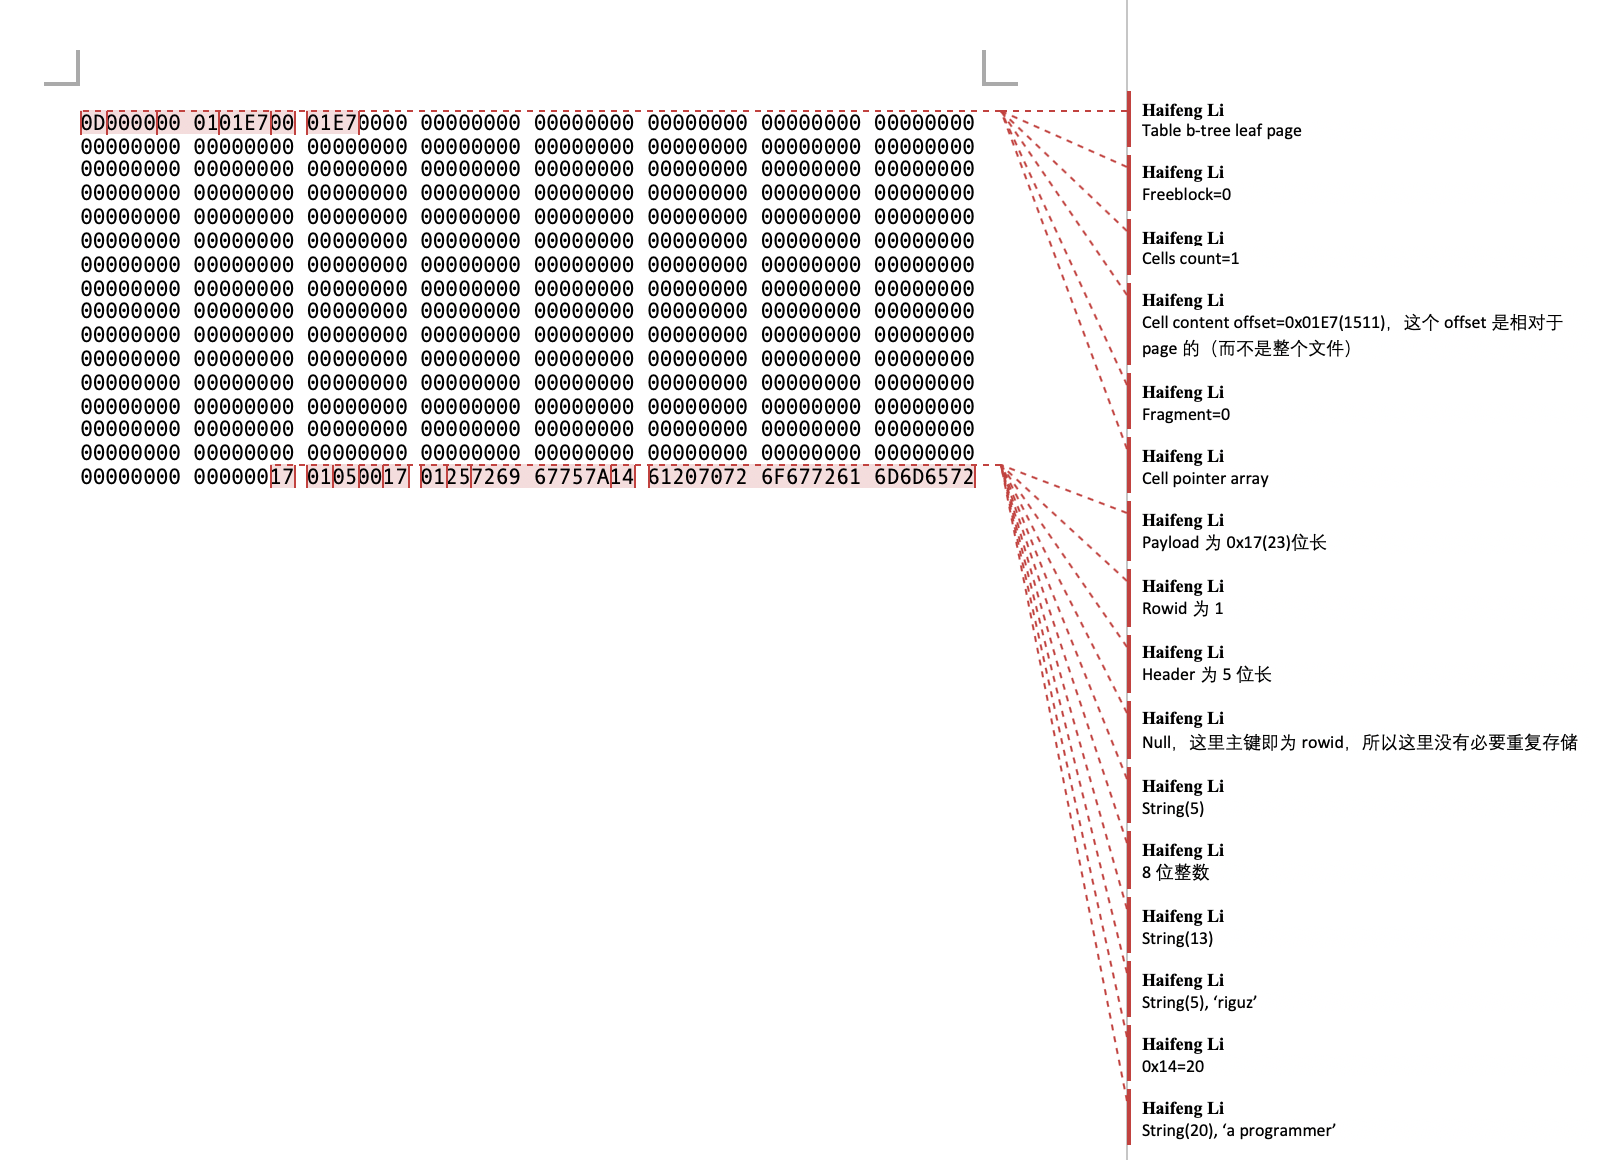
\includegraphics[keepaspectratio,alt={Example}]{images/Sqlite3-rowformat-e1.png}}
\caption{Example}
\end{figure}

一直向表中插入数据，

\begin{Shaded}
\begin{Highlighting}[]
\KeywordTok{insert} \KeywordTok{into}\NormalTok{ person }\KeywordTok{values}\NormalTok{(}\DecValTok{1}\NormalTok{, }\StringTok{\textquotesingle{}riguz1\textquotesingle{}}\NormalTok{, }\DecValTok{20}\NormalTok{, }\StringTok{\textquotesingle{}a programmer\textquotesingle{}}\NormalTok{);}
\KeywordTok{insert} \KeywordTok{into}\NormalTok{ person }\KeywordTok{values}\NormalTok{(}\DecValTok{2}\NormalTok{, }\StringTok{\textquotesingle{}riguz2\textquotesingle{}}\NormalTok{, }\DecValTok{20}\NormalTok{, }\StringTok{\textquotesingle{}a programmer\textquotesingle{}}\NormalTok{);}
\KeywordTok{insert} \KeywordTok{into}\NormalTok{ person }\KeywordTok{values}\NormalTok{(}\DecValTok{3}\NormalTok{, }\StringTok{\textquotesingle{}riguz3\textquotesingle{}}\NormalTok{, }\DecValTok{20}\NormalTok{, }\StringTok{\textquotesingle{}a programmer\textquotesingle{}}\NormalTok{);}
\KeywordTok{insert} \KeywordTok{into}\NormalTok{ person }\KeywordTok{values}\NormalTok{(}\DecValTok{4}\NormalTok{, }\StringTok{\textquotesingle{}riguz4\textquotesingle{}}\NormalTok{, }\DecValTok{20}\NormalTok{, }\StringTok{\textquotesingle{}a programmer\textquotesingle{}}\NormalTok{);}
\KeywordTok{insert} \KeywordTok{into}\NormalTok{ person }\KeywordTok{values}\NormalTok{(}\DecValTok{5}\NormalTok{, }\StringTok{\textquotesingle{}riguz5\textquotesingle{}}\NormalTok{, }\DecValTok{20}\NormalTok{, }\StringTok{\textquotesingle{}a programmer\textquotesingle{}}\NormalTok{);}
\KeywordTok{insert} \KeywordTok{into}\NormalTok{ person }\KeywordTok{values}\NormalTok{(}\DecValTok{6}\NormalTok{, }\StringTok{\textquotesingle{}riguz6\textquotesingle{}}\NormalTok{, }\DecValTok{20}\NormalTok{, }\StringTok{\textquotesingle{}a programmer\textquotesingle{}}\NormalTok{);}
\KeywordTok{insert} \KeywordTok{into}\NormalTok{ person }\KeywordTok{values}\NormalTok{(}\DecValTok{7}\NormalTok{, }\StringTok{\textquotesingle{}riguz7\textquotesingle{}}\NormalTok{, }\DecValTok{20}\NormalTok{, }\StringTok{\textquotesingle{}a programmer\textquotesingle{}}\NormalTok{);}
\KeywordTok{insert} \KeywordTok{into}\NormalTok{ person }\KeywordTok{values}\NormalTok{(}\DecValTok{8}\NormalTok{, }\StringTok{\textquotesingle{}riguz8\textquotesingle{}}\NormalTok{, }\DecValTok{20}\NormalTok{, }\StringTok{\textquotesingle{}a programmer\textquotesingle{}}\NormalTok{);}
\KeywordTok{insert} \KeywordTok{into}\NormalTok{ person }\KeywordTok{values}\NormalTok{(}\DecValTok{9}\NormalTok{, }\StringTok{\textquotesingle{}riguz9\textquotesingle{}}\NormalTok{, }\DecValTok{20}\NormalTok{, }\StringTok{\textquotesingle{}a programmer\textquotesingle{}}\NormalTok{);}
\KeywordTok{insert} \KeywordTok{into}\NormalTok{ person }\KeywordTok{values}\NormalTok{(}\DecValTok{10}\NormalTok{, }\StringTok{\textquotesingle{}riguz10\textquotesingle{}}\NormalTok{, }\DecValTok{20}\NormalTok{, }\StringTok{\textquotesingle{}a programmer\textquotesingle{}}\NormalTok{);}
\KeywordTok{insert} \KeywordTok{into}\NormalTok{ person }\KeywordTok{values}\NormalTok{(}\DecValTok{11}\NormalTok{, }\StringTok{\textquotesingle{}riguz11\textquotesingle{}}\NormalTok{, }\DecValTok{20}\NormalTok{, }\StringTok{\textquotesingle{}a programmer\textquotesingle{}}\NormalTok{);}
\KeywordTok{insert} \KeywordTok{into}\NormalTok{ person }\KeywordTok{values}\NormalTok{(}\DecValTok{12}\NormalTok{, }\StringTok{\textquotesingle{}riguz12\textquotesingle{}}\NormalTok{, }\DecValTok{20}\NormalTok{, }\StringTok{\textquotesingle{}a programmer\textquotesingle{}}\NormalTok{);}
\KeywordTok{insert} \KeywordTok{into}\NormalTok{ person }\KeywordTok{values}\NormalTok{(}\DecValTok{13}\NormalTok{, }\StringTok{\textquotesingle{}riguz13\textquotesingle{}}\NormalTok{, }\DecValTok{20}\NormalTok{, }\StringTok{\textquotesingle{}a programmer\textquotesingle{}}\NormalTok{);}
\KeywordTok{insert} \KeywordTok{into}\NormalTok{ person }\KeywordTok{values}\NormalTok{(}\DecValTok{14}\NormalTok{, }\StringTok{\textquotesingle{}riguz14\textquotesingle{}}\NormalTok{, }\DecValTok{20}\NormalTok{, }\StringTok{\textquotesingle{}a programmer\textquotesingle{}}\NormalTok{);}
\KeywordTok{insert} \KeywordTok{into}\NormalTok{ person }\KeywordTok{values}\NormalTok{(}\DecValTok{15}\NormalTok{, }\StringTok{\textquotesingle{}riguz15\textquotesingle{}}\NormalTok{, }\DecValTok{20}\NormalTok{, }\StringTok{\textquotesingle{}a programmer\textquotesingle{}}\NormalTok{);}
\KeywordTok{insert} \KeywordTok{into}\NormalTok{ person }\KeywordTok{values}\NormalTok{(}\DecValTok{16}\NormalTok{, }\StringTok{\textquotesingle{}riguz16\textquotesingle{}}\NormalTok{, }\DecValTok{20}\NormalTok{, }\StringTok{\textquotesingle{}a programmer\textquotesingle{}}\NormalTok{);}
\KeywordTok{insert} \KeywordTok{into}\NormalTok{ person }\KeywordTok{values}\NormalTok{(}\DecValTok{17}\NormalTok{, }\StringTok{\textquotesingle{}riguz17\textquotesingle{}}\NormalTok{, }\DecValTok{20}\NormalTok{, }\StringTok{\textquotesingle{}a programmer\textquotesingle{}}\NormalTok{);}
\KeywordTok{insert} \KeywordTok{into}\NormalTok{ person }\KeywordTok{values}\NormalTok{(}\DecValTok{18}\NormalTok{, }\StringTok{\textquotesingle{}riguz18\textquotesingle{}}\NormalTok{, }\DecValTok{20}\NormalTok{, }\StringTok{\textquotesingle{}a programmer\textquotesingle{}}\NormalTok{);}
\end{Highlighting}
\end{Shaded}

当插入到第18条数据的时候，split了节点，如图：

\begin{figure}
\centering
\pandocbounded{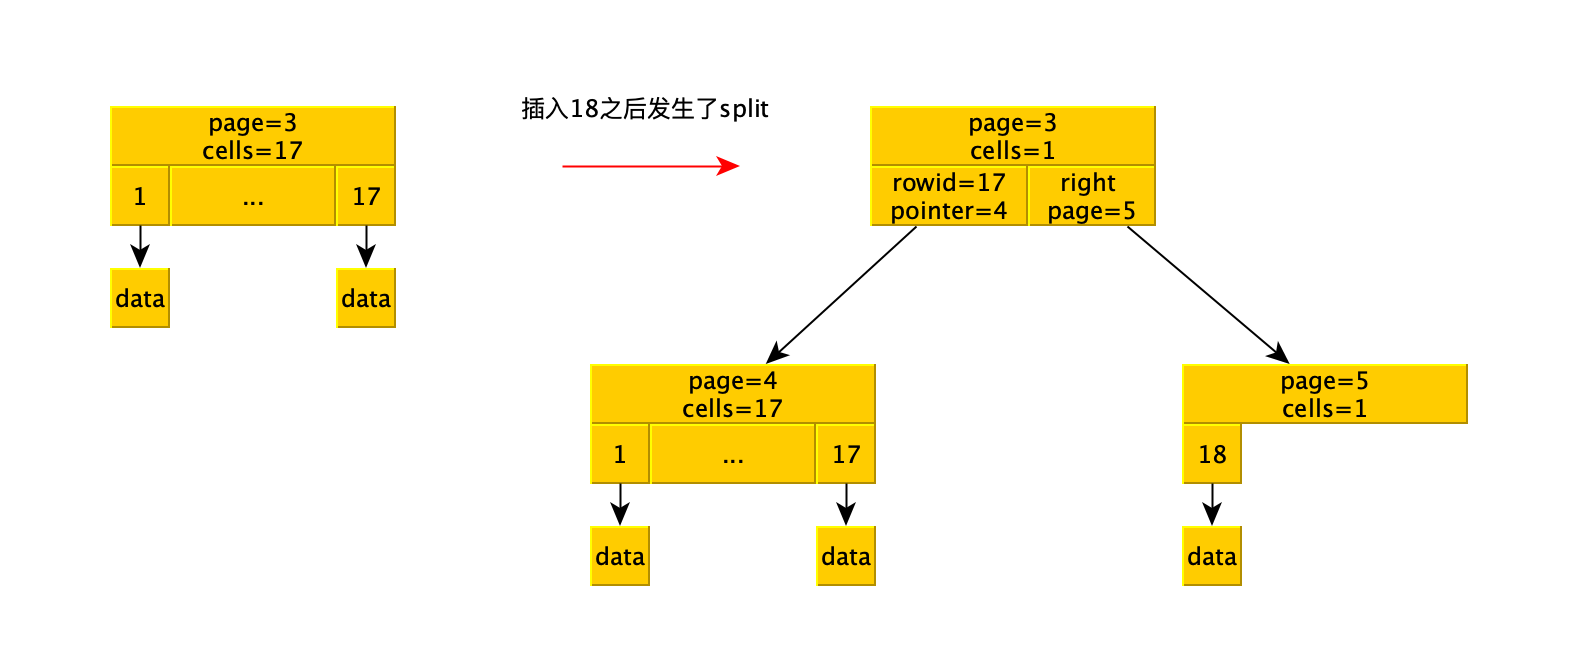
\includegraphics[keepaspectratio,alt={Sqlite split}]{images/Sqlite-split-18.png}}
\caption{Sqlite split}
\end{figure}

\href{https://www.sqlite.org/fileformat.html}{Database File Format} \href{http://barbra-coco.dyndns.org/sqlite/fileformat.html}{}


\end{document}
